\documentclass{article}
\usepackage{graphicx}
\usepackage{amsmath} 
\usepackage{amssymb}
\usepackage{float}
\usepackage{algorithm}
\usepackage{algpseudocode}
\usepackage{subcaption}
%--------- litteratur
\usepackage{natbib}
%---------- 

%---------- hyperref til hyperlink af litteratur
\usepackage[colorlinks=true, linkcolor=blue, citecolor=blue, urlcolor=blue]{hyperref}
%-----------

\title{Bachelor Project 2025}
\author{Johan Søvndahl Kok & Conrad Lavesen Valentinus}
\date{February 2025}
% --------- Fodnoter og litteratur ------

% -------- fodnoter og litteratur -------

\begin{document}
\maketitle
\pagenumbering{roman}
\setcounter{page}{1} 

\newpage
\section*{Abstract}



\newpage
\tableofcontents
\newpage

\pagenumbering{arabic} % Sets page numbering to arabic (1, 2, 3, ...)
\setcounter{page}{1} 

\section{Introduction}

\section{Economic Theory}
HAL R. Varian "Intermediate Microeconomics with calculus"
\newline 
The “Cournot-Bertrand Debate”:
A Historical Perspective 
https://competitionandappropriation.econ.ucla.edu/wp-content/uploads/sites/95/2020/12/CournotBertrand-debate.pdf
Jean Magnan de Bornier 
\newline

In the following section we will focus on unraveling the Economic theory behind the dynamics of the game we will be simulating. 
The overall idea is that we are using machine learning to simulate price competition between two firms. This is being done using a reinforcement learning algorithm known as Q-learning in a duopoly setting known from a Bertrand economy. This framework is based on an article from \cite{Klein2021}, who uses the work of \cite{MaskinTirole} as the economic base for the model. Therefore it is a dynamic, sequential setting, where the firms will take turns of setting their price.
Like \cite{Klein2021}, we will investigate whether using algorithmic pricing can lead to, what can be seen as collusive behaviour.
\newline
We are investigating the dynamics of the game and specifically what happens when you change the number of prices that each firm can set.
\newline



\subsection {Game Theory}
\label{GameTheory}
Game theory, broadly speaking, is a way to provide a framework for trying to understand how rational agents make decisions in individual and group settings, when agents' payoffs depend on their own and other choices.(TADELIS)
\newline
The framework of the simulations in our project are based on game theory. Therefore, we will now introduce project-relevant definitions from game theory and assumptions which will be used when setting up our simulations.
\newline
First off, agents (or players), will be referred to as firms, and are assumed to be rational, meaning that they act according to the actions which maximizes their payoff (TADELIS). The firms' objective is therefore to maximize profits.
\newline
Firms can choose to set different prices when playing against each other. Thus, setting prices are the actions that the firms can take.
The set of actions is called a 'strategy', when we analyze the setting from a game theory perspective. With different strategies, we can end up with different equilibria.
\subsubsection{Nash Equilibrium, SPNE and MPE}
A \textbf{Nash equilibrium} is a strategy or set of strategies in a game where no agent has any incentive to deviate from their strategy, given what the other agents are playing. This ensures that in equilibrium, each agent's strategy is a best response to the other's (\cite{tadelis}).
\newline
In our simulation we are playing a repeated game, which leads us to the definition of the Subgame Perfect Nash Equilibrium (SPNE). A SPNE is a refinement of the Nash equilibrium and means that every subgame of the game is a Nash equilibrium \citep[p. 157]{tadelis}. 
\newline
In a dynamic game like ours, the number of possible subgames is very large. To simplify analysis, \cite{MaskinTirole} introduced the concept of a \textbf{Markov-perfect equilibrium (MPE)} which will be further explained in section \ref{economic Environment}. 


\subsection{Bertrand competition}
The overall competition framework used in the project, will be based on the ideas of Joseph Louis François Bertrand. In a market for a homogeneous good, sold by symmetric firms, Bertrand came up with the theory, that the firms will only be setting the price while the market then will be determining the quantity sold(VARIAN). Bertrand's logic can be used on oligopolies, but as Bertrand originally framed his arguments in 1883 (Jean Magnan De Bornier), this project will be in the setting where only 2 firms exist on the market, namely duopoly. 
\newline
The reasoning for choosing our setting as a duopoly follows from the settings of \cite{MaskinTirole} and thereby \cite{Klein2021}. The ideas of price cycles such as Edgeworth cycles or the case of focal pricing, are described for two firms. Therefore, it is sensible that our setting is also based on two firms, such that we can analyze the dynamics that arises from our model.
Furthermore, we are investigating the dynamics of what happens when we change the number of price points, meaning the number of different prices that the firms can set (will be referred to as the parameter \textit{k}). It is therefore computationally heavy when you introduce more than two firms in the simulation, as the computations needed to be done rises with the parameter \textit{k}.  
\newline
Bertrand originally showed that under all the assumptions above and an assumption of constant cost, the Bertrand equilibrium is when the price is equal to the marginal cost, which is also a Nash equilibrium. However, in markets with few sellers, firms do not typically sell their goods at the marginal cost. 
\cite{MaskinTirole} partly blame this on the fact that the original model proposed by Bertrand was static, meaning that both firms set their prices simultaneously without knowing what the other firm set as a price, and the market clears and the game ends. They argue that having a dynamic model may be important to capture the dynamics of actual price competition (\cite{MaskinTirole}).
In a dynamic model, firms set prices in multiple rounds. This is important for us, as we are investigating the dynamics of price competition.  
\newline
As mentioned before, our model is a dynamic and sequential. \cite{Klein2021} argues that a sequential dynamic model is a more realistic model to capture pricing competition from the real world.
Other researchers, such as \cite{Calvano} have used a simultaneous dynamic setting, where firms play a repeated game, but set their prices in each turn at the same time. We believe that the sequential dynamic setting used in \cite{Klein2021} is more representative of the real world, as it is unlikely that firms always would set prices on the same goods, at exactly the same time. In a duopoly, it's more realistic to assume that one firm sets its price first, the second firm then observes this and sets its own price in response, and finally, the first firm adjusts its price again based on the second firm's price.





\subsection{Economic environment}
\label{economic Environment}
Our model, which is based on \cite{Klein2021}'s sequential pricing duopoly, uses Q-learning in a simulation setting, which we will also do.
We will now further describe the economic environment, which is based on the work of \cite{Klein2021}. 
\newline
Two firms, \textit{i} and \textit{j} take turns on setting prices in infinitely repeated discrete time indexed by $t = \{1,2,3,... \} $. Thus, firm \textit{i} sets price $p_{i,t}$ and firm \textit{j} sets the price $p_{j,t}$ in period \textit{t}. 
The prices that the firms can choose are discrete, evenly spaced and between 0 and 1. The number of different prices that the firms can set are determined by \textit{k}, such that the price interval is denoted by $P = \{0, \frac{1}{k}, \frac{2}{k}, \frac{3}{k},...,1\} $. Prices are set sequentially, such that in even time periods firm $p_i$ sets their price, and in odd time periods $p_j$ sets their price.
\newline
Assuming no marginal or fixed costs, the profit function for firm \textit{i}, in time period \textit{t} is described as:
\begin{equation}
    \pi_i (p_{it},p_{jt}) = p_{it}D_{it}(p_{it},p_{jt})
\end{equation}
where $p_{jt}$ is the price of the opposite firm, and $D_{it}$ is the demand as a function of its own price $p_{it}$, and the price of the opposing firm, $p_{jt}$.
Firms discount future profits with $\delta \in [0,1)$, such that it is the objective of each firm to maximize, at time \textit{t}, the following:
\begin{equation}
\max\sum_{s=0}^{\infty}\delta^s\pi_i(p_{i,t+s},p_{j,t+s})
\end{equation}
\newline
The demand function is defined as:
\begin{equation}
D_i(p_{it},p_{jt}) =
\begin{cases}
  1-p_{it} &\text{if } p_{it} < p_{ij},\\
  \frac{1-p_{ij}}{2}   & \text{if } p_{it} =p_{ij},\\
  0   & \text{if } p_{it} > p_{ij}
\end{cases}
\end{equation}
Which means that the firm with the lower price takes the whole market. If both firms set the same price, they split the market evenly. 





The monopolist's profit corresponds to the joint-profit maximizing profit. Therefore, we calculate the monopolist's profit, such that it can later be used as a benchmark. This allows for a clearer interpretation of the profit levels observed in the simulation, by comparing them to the theoretical maximum achievable profit through full cooperation.
\newline
The monopolist's demand function is:
\begin{equation}
    D(p) = 1-p
\end{equation}
with a profit of
\begin{equation}
    \pi (p) = p \cdot D(p) = p \cdot (1-p) \Leftrightarrow \pi (p) = p - p^2
\end{equation}
maximizing over p, we take the derivate with respect to p: 
\begin{equation}
    \cfrac{d \pi(p) }{d p} = 1-2p
\end{equation}
and now setting the equation equal to 0 and isolate for p:
\begin{equation}
    0 = 1 - 2p \Leftrightarrow p = \cfrac{1}{2}
\end{equation}
Which means that the joint-profit maximizing price is:
\begin{equation}
    p^M = 0.5
\end{equation}
with a profit for each firm of:
\begin{equation}
\label{MonopolistPrice}
\pi_{ij}^M (p^M) = 0.5 \cdot \cfrac{1 - 0.5}{2} = 0.125
\end{equation}
\label{Joint_profit_price}
\newline
Following the works of \cite{Klein2021} and \cite{MaskinTirole}, we impose the Markov assumption: only directly relevant payoffs are used to determine the strategy of the firms. This means that the strategy that the firms follow, are only dependent on the price that the other firm set in the last period $p_{j,t-1}$. This implies that the history of the prices (other than the last period) are irrelevant, and that there is no communication between the firms.
As mentioned in section \ref{GameTheory}, strategies are the prices that the firms are setting.
\newline
Because we are in a dynamic environment, we will define what will be an equilibrium in this setting. 
The following value function is a Nash equilibrium for all prices along the equilibrium path, if the condition holds for both firms:
\begin{equation} \label{KleinBellmanEq}
    V_i(p_{jt}) = \mathop{\text{max}}_{\text{p}} [\pi_i (p,p_{jt}) + E_{p_{j,t+1}}[\delta \pi_i (p,p_{j,t+1})+\delta^2 V_i (p_{j,t+1}) ]]
\end{equation}
Equation (\ref{KleinBellmanEq}) is written in the style of \cite{Klein2021}, who has the equation from \cite{MaskinTirole}. They introduce the concept of a Markov Perfect Equilibrium (MPE). An MPE is a special type of SPNE where the strategy of each player depends only on the current “state” of the game — not the full history. This is known as the \textbf{Markov assumption}, and in our model, the state is simply the price set by the opponent in the previous round.
If you include off-equilibrium prices, for all prices a strategy pair $(R_1,R_2)$ is MPE if equation (\ref{KleinBellmanEq}) holds.

\subsubsection{Edgeworth Price Cycles and Focal Pricing} \label{EdgeworthFocalpricingSec}
Further, \cite{MaskinTirole} show that if firms value future profits sufficiently \footnote{When \cite{MaskinTirole} talk about valuing future profits 'sufficiently' high with a 'sufficiently' high discount factor, they mention one close to 1, without giving a specific number. An idea of a sufficiently high discount factor is calculated to be ??0.877?? in the works of KILDE?!?!??!?!??!}, two kinds of MPE's exist, 
namely focal pricing and Edgeworth price cycles.
Focal pricing is when both firms are playing the same price, repeatedly. This equilibria exists because of the fear from the firms, that if they undercut their competitor, that the competitor would follow suit and undercut them aswell. This would start a price war, which would be costly for the firms. And because they value future profit sufficiently, none of the firms are willing to start this price war. Similarly, the firms are not willing to increase the price, as they believe that the other firm would not follow, and then they would lose the entire market.
\newline
Edgeworth price cycles are when firms gradually undercut each other, to increase market share, until the price war becomes too costly (price reaches marginal cost, which in our case is 0), and one of the firms resets the price to a 'high' price (one increment above the monopoly price), and the undercutting begins again (\cite{MaskinTirole}). In this way, a cycle pattern arises, which can be seen in Figure \ref{fig:EdgeworthCycle}.

\begin{figure}[H]
    \centering
    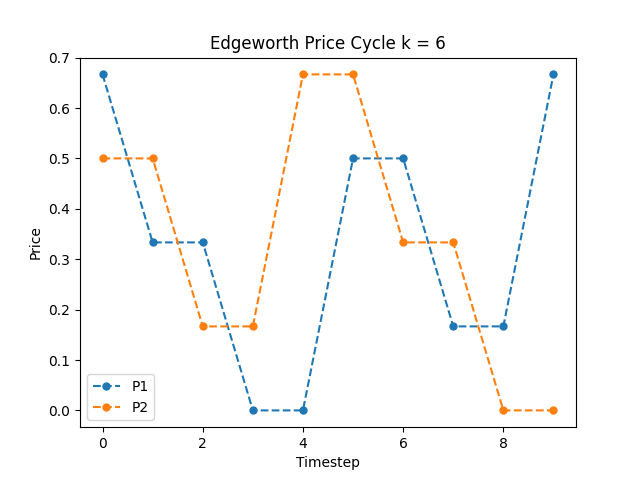
\includegraphics[scale = 0.75]{Edgeworth price cycle k = 6.png}
    \caption{Edgeworth price cycle for two firms with \textit{k} = 6. Firms undercut each other until the first firm to observe the lowest price resets the price cycle. In this case firm 2 are the first to reset the cycle, and then the next reset is done by firm 1.}
    \label{fig:EdgeworthCycle}
\end{figure}
The Edgeworth price cycle changes, as the price interval changes (number of prices that the firms can set, denoted by parameter \textit{k}). This is important to note, as we will later analyze what happens when \textit{k} changes. 
\newline
We simulate the Edgeworth cycles with different values for \textit{k} in Python, and calculate the per period profit corresponding to the Edgeworth cycle with a given \textit{k}.
The per period profit of the Edgeworth price cycle will serve as a benchmark for the competitive level of profit, just as it does in \cite{Klein2021}. For $k = 6$, the per period profit is $\pi = 0.0611$. Note that other candidates for the competetive benchmark are the static Nash outcome of the game where both firms set the price at the marginal cost (or one increment above the marginal cost), both of which is a static Nash equilibrium. However, due to the dynamics of the game, the static Nash outcome is not a suitable benchmark for a repeated game (\cite{Klein2021}).
\newline
As we are investigating what happens when \textit{k} changes, we need to calculate the per period profit of the Edgeworth cycles. This is done using our Python script and the results are reported in table (\ref{tab:kPrPeriodProf})

\begin{table}[H]
    \centering
    \begin{tabular}{|c|c|}
        \hline
        Size of price interval, \textit{k} & Per period profit of the Edgeworth cycle \\
        \hline
        k = 6 & 0.0611 \\
        \hline
        k = 12 & 0.0699 \\
        \hline 
        k = 24 & 0.0758 \\
        \hline
        k = 48 & 0.0793 \\
        \hline
        k = 100 & 0.0813 \\
        \hline
    \end{tabular}
    \caption{The per period profit associated with the Edgeworth price cycle for different values of \textit{k}.}
    \label{tab:kPrPeriodProf}
\end{table}




\section{Reinforcement learning theory} \label{ReinforcementLearningTheory}

\subsection{Introduction to Reinforcement Learning}
Reinforcement learning (RL) is a concept from machine learning, that differs from other types such as supervised learning and unsupervised learning.
Supervised learning is where you have labeled input-output pairs, and the objective is then to find the unknown function which this data is from. An example of supervised learning could be the very well-known OLS regression which tries to fit a linear model to data. In unsupervised learning, you have access to unlabeled data, and the objective is to find patterns or structures. An example of unsupervised learning could be K-means clustering which tries to find clusters in unlabeled data, thereby finding patterns. RL differs from these methods, and instead learns the most optimal choices through repeated interactions with the environment. This is therefore a 'trial and error' approach, where the algorithm tries new actions, and learns through which actions give the best rewards. A great and relevant example of an RL algorithm would be Q-learning (MARL side 19-21). \citep[p. 19-21]{MARLBOOK}
\newline 
\newline
A more general definition of RL is provided in the book "Multi-Agent Reinforcement Learning:
Foundations and Modern Approaches" by Stefano V. Albrecht,  Filippos Christianos,  Lukas Schäfer, which will also serve as a primary source for this theory section and corresponding subsections. The definition: 
"\textbf{Reinforcement learning (RL) algorithms learn solutions for sequential
decision processes via repeated interaction with an environment.}"
From the definition it is clear where RL get its "trial and error" reputation.   
\newline
(MARL side 20)
\newline
\newline
A sequential decision process is when an agent inside an environment makes decisions and observes one time step at the time. To define sequential decision processes, a decision process model is needed to guide the decisions, and a learning objective must be established to evaluate each strategy. Together, the model and objective constitute a reinforcement learning problem, as shown in Figure \ref{fig:MARLside20} (MARLside20). In relation to our thesis, we use Markov Decision Processes (MDP) as the decision process model for our Q-learning implementation.
\newline 
\newline
The environments in which we implement our RL algorithms determine whether we are dealing with Multi-Agent RL or Single-Agent RL. The two concepts of Single and Multi-agent RL will be elaborated upon later, but to quickly summarize: Single-agent RL interacts with an environment alone, while  Multi-agent acts with an environment with other agents. (MARL SIDE 19-21).
In this section, we will unpack the theory essential to understanding the underlying principles of Q-learning, beginning with the single-agent framework and MDP, trying to translate the general Q-learner setup to our Economic environment. 
\begin{figure}
    \centering
    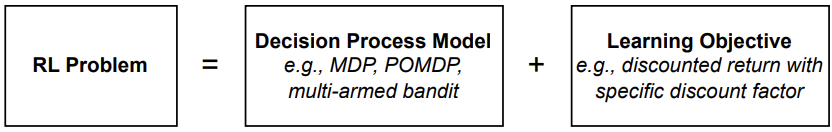
\includegraphics[width=0.5\linewidth]{MARLside20.png}
    \caption{Figure from MARL side 20 }
    \label{fig:MARLside20}
\end{figure}
\subsection{Single Agent Reinforcement Learning}
In this subsection we will be attacking the theory of RL in the Single-agent approach, many of the following concepts that will be introducet  lay the groundworks ....
\subsubsection{Markow Decision Processes}
As metioned earlier, Markov Decision Processes (MDP) will be the Decision Process Model that we will focus on. It serves as the standard model for sequential decision processes that lays the foundation for
defining Single-Agent RL (MARL side 19-22). This can be said in more intuitive terms: MDP provides a structured way to model the process where an agent must make a series of decisions over time in an environment.
\newline
\textbf{Definition 1: Markov Decision Process MARL SIDE 22} A Discrete (MDP) consists of:
\begin{enumerate}
    \item \textbf{Finite set of states \( S \)}, with a subset of terminal states \( \bar{S} \subset S \).
    \item \textbf{Finite set of actions \( A \)}.
    \item \textbf{Reward function \( \mathcal{R}: S \times A \times S  \to \mathbb{R} \)}.
    \item \textbf{State transition probability function \( \mathcal{T}: S \times A \times S \to [0, 1] \)} such that
    \[
    \forall s \in S, a \in A : \sum_{s' \in S} \mathcal{T}(s, a, s') = 1 \quad 
    \]
    \item \textbf{Initial state distribution \( \mu: S \to [0, 1] \)} such that
    \[
    \sum_{s \in S} \mu(s) = 1 \quad \text{and} \quad \forall s \in \bar{S}, \mu(s) = 0 \quad 
    \]
\end{enumerate}
Let us now try to explain exactly what this mean starting with the first item of the definition.
\newline 
\textbf{Finite set of state S} represents all the possible situations an agent can be in. In our case, a firm's state is determined by the price set by its competitor. Instead of defining specific terminal states, where the agent stops acting, we ensure that the simulation ends by imposing a maximum number of time steps, which serves the same purpose and is the approach we use in our simulations.
\newline
A \textbf{Finite set of actions A} are the possible actions that an agent would have. In our case this is the firm's different options for setting the price, which is determined by the parameter \textit{k}. 
\newline
The \textbf{Reward function} determine the reward of an action and thereby how well the action was guiding the agent. In our case, this will be a profit function. 
\newline
The \textbf{State Transition probability function's} goal is to explain how the environment changes. It can be thought of like a rulebook, containing rules of the game. The state transition probability function only have a theoretical relevance to this thesis, which will be made clear in section \ref{Temporal Difference Learning and Q-learning}. 
\newline
The \textbf{Initial State Distribution} defines the probabilities of the agent being in a particular state at the beginning of the game. For example, if a firm has two possible starting states $s_1$ and $s_2$ (which would be determined by a \textit{k} value of 2), the initial state distribution might look like $s_1=30\%$ and $s_2 = 70\%$ meaning there's a $30\%$ chance the firm starts in state $s_1$ and a $70\%$ chance it starts in state $s_2$.
\newline 
\newline 
One could easily think that the Markow Decision process could have something to do with the Markow assumption, also known as the Markow property mentioned in section \ref{GameTheory}, and indeed it does. 
As we know, the Markow assumption says that the future state (competitor price) and reward (profit) are conditionally independent of past states (competitor prices) and actions (own prices), when you have the current state (competitor price) and action (own price). Mathematically the assumption is expressed in equation \ref{Markow_property}.
\begin{equation}
\label{Markow_property}
P(s_{t+1}, r_t | s_t, a_t, s_{t-1},a_{t-1} \dots, s_0, a_0) = P(s_{t+1}, r_t | s_t, a_t)
\end{equation}
This allows us to only give an agent the current state and it would still be sufficient information for it to take optimal actions in an MDP. 
Limiting the agent therefore limits the amount of complex coding and makes the process less computationally demanding, by not needing to store and use past states and actions. (MARL side 23)
\subsubsection{Value functions and Bellman equation}
YAP YAP YAP introduction til denne her del:
Moving forward we will have to define a strategy function, that returns a probability from which the MDP chooses an action conditioned on the state. It will be denoted as: $\mathcal{P}(a_t,s_t)$. When working with MDP, one can define a solution a as optimal strategy $\mathcal{P}^*$, which is the strategy that results in the maximum expected discounted return. 
To determine which strategy does exactly this we will use the Bellmann Equation, also known as the state value function, which can be seen in equation )\ref{bellmann-equation})
\begin{equation}
    \label{bellmann-equation}
    V^{\mathcal{P}}(s)= \sum_{a\in A}\mathcal{P}(a|s)\sum_{s'\in S}\mathcal{T}(s'|s,a)[\mathcal{R}(s,a,s')+\delta V^{\mathcal{P}}(s')]
\end{equation}
Where s' denotes the future states and $\delta$ is the discounting parameter. 
The purpose of equation (\ref{bellmann-equation}) is to give the expected return when selecting actions with strategy $\mathcal{P}$, starting in state s. From the same logic, we can now define the action value function $Q^{\mathcal{P}}(a,s)$ in equation (\ref{action_value_func}).
\begin{equation}
    \label{action_value_func}
    Q^{\mathcal{P}}(a,s)=\sum_{s'\in S}\mathcal{T}(s'|s,a)[\mathcal{R}(s,a,s')+\delta\sum_{a'\in A}\mathcal{P}(s|a')Q^{\mathcal{P}}(a',s')]
\end{equation}
$Q^{\mathcal{P}}(a,s)$ returns the expected value but this time selecting an action a in state s and then following strategy $\mathcal{P}$ to select actions afterwards.
Since we are in the MDP, the strategy is optimal if its corresponding value function is optimal. This then leads us to Bellman Optimality Equations which can without needed reference to the strategy functions because...., where * denotes optimality:
\begin{equation}
    \label{V_optimal}
    V^*(s) = \max_{a\in A}\sum_{s'\in S}\mathcal{T}(s'|s,a)[\mathcal{R}(s,a)+\delta V^*(s')]
\end{equation}
\begin{equation}
    \label{Q_optimal}
    Q^*(s,a)= \sum_{s'\in S}\mathcal{T}(s'|s,a)[\mathcal{R}(s,a,s')+\delta \max_{a'\in A}Q^*(s',a')]
\end{equation}
Equations \ref{V_optimal} and \ref{Q_optimal} illustrates that the optimal strategy in an MDP relies on the optimal value function. To find the optimal strategies for given states, we select actions that maximize the value, as shown in equation \ref{Optimal_strategy}.
\begin{equation}
    \label{Optimal_strategy}
    \mathcal{P}^*(s) =  \arg \max_{a \in A}Q^*(s,a)
\end{equation}
Two families of algorithms are used to calculate optimal value functions and thereby optimal strategies, respectively Dynamic programming and Temporal Difference learning. While Dynamic Programming estimates value functions using complete knowledge of the MDP, Temporal difference learning updates value estimates based on interactions with the environment, making the latter of relevance to Q-learning and by extension our thesis. 
MARL SIDE 26-28
\subsubsection{Temporal difference Learning and Q-learning}
\label{Temporal Difference Learning and Q-learning}
Temporal difference learning (TD) is a family inside the world of RL where value functions and optimal strategies are learned through experiences which are generated in the following loop: An agent choose an action, to which the environment responds by modifying the state, which the agent then observes through a reward function and responds to by choosing an action. In the following, the reward function $\mathcal{R}(s^t,a^t,s^{t+1})$ will simply be denoted as $r^t$. As mentioned above, TD learning relies on interactions with the environment and does not require full knowledge of the Markov Decision Process. This makes the state transition function unnecessary. As a result, we can modify the Bellman optimality equations, originally shown in equations (\ref{V_optimal}) and (\ref{Q_optimal}) to the equations (\ref{TD_V_optimal}) and (\ref{TD_Q_optimal}).
\begin{equation}
    \label{TD_V_optimal}
        V^*(s) = \max_{a\in A}[r^{t+1}+\delta V^*(s^{t+1})]
\end{equation}

\begin{equation}
    \label{TD_Q_optimal}
        Q^*(s,a)= [r^{t+1}+\delta \max_{a'\in A}Q^*(s^{t+1},a')]
\end{equation}
In temporal difference learning, the update rule for learning the action value function $Q(s,a)$, uses equation (\ref{TD_Q_optimal}) and is shown in equation (\ref{TD_update_Q}) just below. 
\begin{equation}
    \label{TD_update_Q}
    Q(s^t,a^t)\leftarrow Q(s^t,a^t)+\alpha *[\underbrace{ r^{t+1}+\delta \max_{a'\in A} Q(s^{t+1},a')}_{\text{Equation \ref{TD_Q_optimal}}}-Q(s^t,a^t)]
\end{equation}
The update rule (equation (\ref{TD_update_Q})) is used to estimate the action value function after interactions with the environment on a given time. 
In the update rule, a new variable $\alpha$ is used, which is the learning rate, also known as step size which lies between the values (0;1]. It can be seen as how much new interactions are weighted against older interactions. Using the theory from above we can now introduce pseudocode for the single agent Q-learning algorithm, showcased Algorithm 1, which uses the update rule from equation (\ref{TD_update_Q}).
\begin{algorithm}[H]
\caption{Q-learning for MDPs using the Epsilon Greedy Strategy Method}
\begin{algorithmic}[1]
\State Initialize: \( Q(s, a) = 0 \) for all \( s \in S, a \in A \)
\State Repeat for every episode:
\For{$t = 0, 1, 2, \dots$}
    \State Observe current state \( s^t \)
    \State With probability \( \epsilon \): choose random action \( a^t \in A \)
    \State Otherwise: choose action \( a^t \in \arg \max_{a} Q(s^t, a) \)
    \State Observe own reward \( r^{t+1} \) and next state \( s^{t+1} \)
    \State \( Q_i(s^t, a^t) \gets Q(s^t, a^t) + \alpha [r^{t+1} + \delta \max_{a} Q(s^{t+1}, a) - Q(s^t, a^t)] \)
\EndFor
\end{algorithmic}
\end{algorithm}
Epsilon-Greedy Strategy Method is a way to making sure the Q-learner explores the action-state space, while still converging to an optimal strategy. The method is shown down below in equation (\ref{epsilongreedy}) 
\begin{equation}
    \label{epsilongreedy}
    a^t\begin{cases}
        \sim\text{U}(A)& \text{with probability $\epsilon^t$}\\
        \arg \max_a Q(s,a) & \text{with probability 1-$\epsilon^t$}
    \end{cases}
\end{equation}
It shows how an action is chosen with a probability determined by $\epsilon$ to either pick a random action from a uniform distribution or an action that maximize the action-value function $Q(s,a)$. This is what happens at line 5-6 in algorithm 1. 
The purpose is to gradually decrease the value of epsilon as the number of time steps increases, reducing the likelihood of exploration over time and making sure that the Q-learner eventually converges toward a strategy.
MARL(side 32-35)
\subsection{Multi Agent Reinforcement Learning}
Now that the section above have given a better understanding of the theory and methods behind how Single-Agent RL works, we will now move onto Multi-Agent RL. The relevance of both having multi agent and single agent RL theory and methods will become clear in the following. Figure \ref{fig:marside44} from MARL page 44 finely illustrates an overview of the Multi-agent RL hierarchy. It illustrates how Repeated Normal-Form games and Markow Decision Processes are special cases of Stochastic Games which are special cases of Partially Observable Stochastic Games. The figure also shows that the number of states and agents classify each type of game. In this thesis we are focusing on Q-learning and Q-learners (agents) playing and learning against each other. The states will be fully observed and transparent for each agent and combining that with having multiple agents working in the same environment means we only will be exploring the Stochastic Games and Markow decision processes.
\begin{figure}[H]
    \centering
    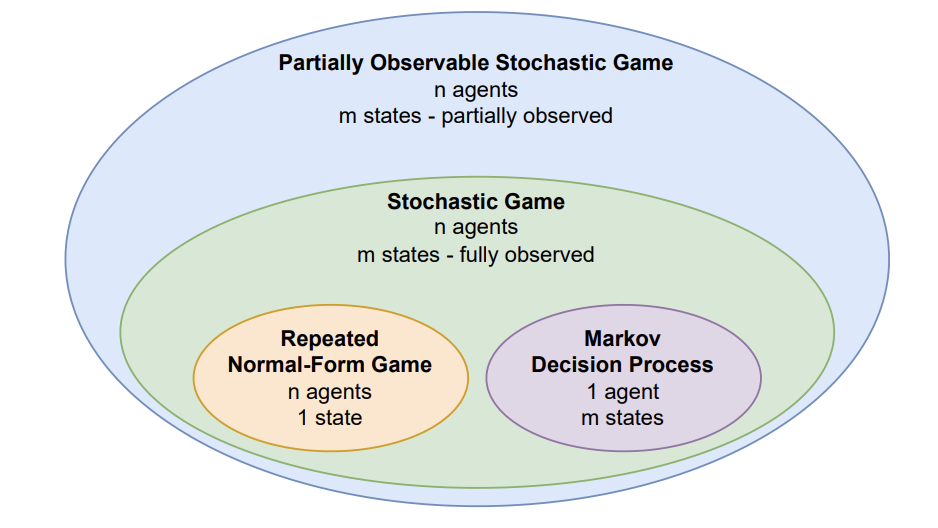
\includegraphics[width=0.5\linewidth]{Multi-agent-figure.png}
    \caption{Multi-Agent RL Hierarchy }
    \label{fig:marside44}
\end{figure}
\subsubsection{Stochastic games and Independent Learning}
Most of the theory that Stochastic games are build upon is very similar to MDP's and therefore to avoid repeating ourselves the following will seem more superficial. A more formal definition of a stochastic game is given in definition 3 from MARL side 47-48. 
\newline
\textbf{Definition 2 (Stochastic game)} A stochastic game consists of:

\begin{enumerate}
    \item Finite set of agents \( I = \{1, \dots, n\} \)
    \item Finite set of states \( S \), with a subset of terminal states \( \bar{S} \subset S \)
    \item For each agent \( i \in I \):
    \begin{itemize}
        \item Finite set of actions \( A_i \)
        \item Reward function \( R_i: S \times A \times S\to \mathbb{R} \), where \( A = A_1 \times \dots \times A_n \)
    \end{itemize}
    \item State transition probability function \( T: S \times A \times S \to [0, 1] \) such that
    \[
    \forall s \in S, a \in A : \sum_{s' \in S} T(s, a, s') = 1
    \]
    \item Initial state distribution \( \mu: S \to [0, 1] \) such that
    \[
    \sum_{s \in S} \mu(s) = 1 \quad \text{and} \quad \forall s \in \bar{S}: \mu(s) = 0
    \]
\end{enumerate}
From the definition it is clear to see that it is just an expansion of the definition (1) of the MDP, with the addition, that it can handle multiple agents in the same environment. It can be seen directly by the indices introduced at point 1, in definition (2). In our thesis the number of agents (firms) will, as mentioned, be 2. Similar to the MDP, the Stochastic games have the same Markow Assumption as shown in equation \ref{Markow_property}. Given these similarities, it comes as no surprise that Stochastic Games are also referred to as Markov Games. (MARL side 48).
\newline 
\newline
Multi-agent RL can be used to learn strategies for handling real-world problems. And since the problems that RL are used to solve differs quite a bit, the approach on how to actually apply the RL also differs quite bit. In this thesis, we will be using the approach of reducing 
a multi-agent RL game into multiple single-agent RL games within the Multi-agent game. This is a standard approach in RL which lowers complexity by reducing the multi-agent learning problem to a single-agent learning problem. More specifically there are 2 different ways to execute this approach, namely Central Learning and Independent Learning. Central Learning is when you take the joint action space for multiple agents and then apply single Agent RL to the joint actions space all together, therefore learning a central strategy that chooses actions for all agents. Central Learning could therefore make sense to use in environments where the agents work together. Independent Learning is when you apply single agent RL to each agent independently, essentially isolating each agent. This means that each agent learns their own independent strategies and ignore the presence of the other agents. They just see the other agents as part of the environment. Independent learning would therefore be a great approach for environments where agents work against each other, which is why this is the approach we have been using in the thesis (Side 95 MARL). 
\newline
\newline
The independent Learning approach to multi-agent Reinforcement Learning brings us to the pseudo code for Independent Q-learning seen in Algorithm 2 (MARL side 98), which is easy to recognize, as it is just an expansion of Algorithm 1. The new thing is again that indices have been introduced to handle multiple agents and their corresponding action and state space.
\begin{algorithm}[H]
\caption{Independent Q-learning (IQL) for stochastic games}
\textbf{Algorithm controls agent \(i\)}
\begin{algorithmic}[1]
\State Initialize: \( Q_i(s_i, a_i) = 0 \) for all \( s_i \in S_i, a_i \in A_i \)
\State Repeat for every episode:
\For{$t = 0, 1, 2, \dots$}
    \State Observe current state \( s_i^t \)
    \State With probability \( \epsilon \): choose random action \( a_i^t \in A_i \)
    \State Otherwise: choose action \( a_i^t \in \arg \max_{a_i} Q_i(s_i^t, a_i) \)
    \State (meanwhile, other agents \( j \neq i \) choose their actions \( a_j^t \))
    \State Observe own reward \( r_i^{t+1} \) and next state \( s_i^{t+1} \)
    \State \( Q_i(s_i^t, a_i^t) \gets Q_i(s_i^t, a_i^t) + \alpha [r_i^{t+1} + \delta \max_{a_i} Q_i(s_i^{t+1}, a_i) - Q_i(s_i^t, a_i^t)] \)
\EndFor
\end{algorithmic}
\end{algorithm}

\subsection{Linking to Economic Environment}
\label{siste Q teori afsnit}
As mentioned in section \ref{economic Environment} the game that we will be simulating in this thesis is between 2 firms. Firm \textit{i} and \textit{j} exist in a sequential duopoly following a bertrand economy, and are competing by setting prices.
By translating the RL theory to the Economic Environment, introduced in section \ref{economic Environment}, we will get the following action and state space and reward function, for firm \textit{i}, while it is symmetrical for firm \textit{j}:
$$A_i = P = \{0, \frac{1}{k}, \frac{2}{k}, \frac{3}{k},...,1\} \text{,  where }p_i\in P$$
$$S_i=P=\{0, \frac{1}{k}, \frac{2}{k}, \frac{3}{k},...,1\} \text{,  where }p_j\in P$$ 
$$\mathcal{R}(a_i,s_i) = \pi_i(p_i,p_j)$$
Therefore, the action space is all of the prices that the firm can set (determined by \textit{k}). The state space is determined by the competitor price, and the size of this space will also be given by \textit{k}. The reward function is determined by the profit function.
\newline
Algorithm 2 shows a way to implement Q-learning using independent learning. In this algorithm the firms are playing each other simultaneously, meaning that they in each time step both are setting a price. 
The decision process we want to simulate is turn-based, between firms since the firms will be taking turns in setting the price against each other as in \cite{Klein2021}. ..... CHATTEN TIL AT UDDYBE.
\newline 
Our simulations will therefore handle this variation of sequential turn-based setting using the following rewards definition inspired by \cite{Julius2023}, who also followed the work of \cite{Klein2021}: 
\begin{equation}
\label{last_reward}
    r_i^{t+1} = \pi_i(p^t_i,p^t_j) + \delta\pi_i(p_i^t,p_j^{t+1})
\end{equation}
The definition shown in \ref{last_reward} equation is tailored to this exact scenario. It takes into consideration that firm \textit{i} is never setting prices in 2 consecutive time steps, by defining its rewards as the direct profit and the profit in the next time step where a new state is introduced, when firm \textit{j} sets a price. $\delta$ discounts the future state profit for one period. Similarly, we also need to adapt the use of the action value function the same way giving us an update rule, which is a modification of equation \ref{TD_update_Q}:
\begin{align}
\label{Klein_update_rule}
Q(p_j^t,p_i^t)\leftarrow Q(p_j^t,p_i^t)+\alpha *[&r_i^{t+1}+\delta^2 \max_{p_i'\in p_i} Q(p_j^{t+1},p_i') -Q(p_j^t,p_i^t)], \\
&r_i^{t+1} = \pi_i(p^t_i,p^t_j)+\delta\pi_i(p_i^t,p_j^{t+1}) \notag 
\end{align}
Again, notice that the Q-value is now discounted for 2 time steps ($\delta^2$), again to handle the sequential turn-based setting.
\newline 
It is also worth noting the similarity between equation (\ref{Klein_update_rule}) and equation (\ref{KleinBellmanEq}). As noted by \cite{Klein2021}, this relationship comes from the fact that Q-learning, via recursive updating, aims to solve a dynamic programming condition.
\newline 
With this new update rule and corresponding game modification we will now show the last algorithm, which is the one we have used for our simulations. Pseudo code for Algorithm 3 can be seen below, which is inspired by \cite{Julius2023}.  
\begin{algorithm}[H]
\caption{Q-learning Sequential Bertrand Duopoly (Greedy $\epsilon$)}
\begin{algorithmic}[1]
\State Initialize: \( Q_i(p_j, p_i) = 0 \textbf{ and } Q_j(p_i, p_j) = 0 \) for all \( p_j, p_i \in P \)
\State Repeat for every episode:
\For{$t = 0, 1, 2, \dots$}
    \State Observe current state (competitor price) \( p_j^t \)
    \State With probability \( \epsilon \): choose random action (price) \( p_i^t \in P \)
    \State Otherwise: choose action (price)  \( p_i^t \in \arg \max_{p_i} Q_i(p_j^t, p_i) \)
    \State Observe next state (competitor price) \( p_j^{t+1} \)
    \State Observe own reward \(r_i^{t+1} = \pi_i(p^t_i,p^t_j)+\delta\pi_i(p_i^t,p_j^{t+1}) \) 
    \State \( Q(p_j^t,p_i^t)\gets Q(p_j^t,p_i^t)+\alpha *[r_i^{t+1}+\delta^2 \max_{p_i'\in p_i} Q(p_j^{t+1},p_i') -Q(p_j^t,p_i^t)]\)
    \State Update $\{i\leftarrow j,j\leftarrow i\}$ \# Other players turn
\EndFor
\end{algorithmic}
\end{algorithm}
Compared to algorithm 2, the algorithm is now using the economic variable names (e.g. states and actions are competitor and own prices, respectively).
Line 1 in algorithm 3, illustrates how the Q values for firm \textit{i} and \textit{j}  are stored in $P\times P$ matrices when computed. All entries in the matrices are initialized as 0, but any arbitrary number would do.
In this way the Q-learning algorithm will try to find the best strategy, given what the opponent is playing.
\newline
Under the right conditions, optimal convergence is guaranteed for a single agent Q-learning problem. However, in our case, such convergence cannot be assured, as the problem has been expanded to a multi-agent setting. One key challenge in this context is the so-called \textit{moving target problem}, which arises when the two agents gradually adapt their strategies. As each agent continuously updates its behavior in response to the other, the optimal strategy becomes a moving target, complicating the learning process.
\section{Setup for simulation}

In this section we will describe how we are running the simulation, and what parameters are being used. 

When running the simulations, we are letting two Q-learners compete against each other, as in the theoretical frame that we set up earlier.

The setup for the simulation is following the work of \cite{Klein2021}. This is done such that results are comparable.
We are running the simulations over $500,000$ timesteps (T=500,000), and then doing that a $1000$ times. In the graphs, the average is a running average taken over $1000$ timesteps each time. This is to smooth out short term fluctuations, where the algorithms are learning, and trying out setting new prices. The average profit in the end is reported as the average profit in the last $1000$ rounds. This is because we are interested to see what level of profit the Q-learning algorithms are making when the algorithms have 'converged'. In the end of the simulation the algorithms have converged (but as mentioned above, this is not guaranteed to be an optimal strategy). The convergence comes from the fact that the exploration parameter decays. More on this in section \ref{Parameters}. 
In our simulation, we chose, in line with \cite{Klein2021}, to view an outcome as 'collusive' if the profit lies over the profit of the competitive benchmark, which is determined by the per period profit from the most profitable Edgeworth cycle (Profits between $p_i = 0.0611$ and $p_i = 0.0813$ for different values of \textit{k}) (Table (\ref{tab:kPrPeriodProf}). Another benchmark that we are using is the per period joint-profit maximizing of $\pi_i =0.125$ from equation (\ref{MonopolistPrice}). This is to give an idea of how 'collusive' the outcome is.

\subsection{Parameters}
\label{Parameters}
If we recall the $\epsilon_t$ it determine the probability of a Q-learner chosing a random action instead of a calculated one given a time step t, therefore calling it the exploration parameter. It is determined by the following equation:
\begin{equation}
\label{eq:epsilon-theta}
    \epsilon_t = (1-\theta)^t 
\end{equation}
Equation \ref{eq:epsilon-theta} makes it such that the algorithm will do a lot of exploration in the beginning, and then gradually decrease. Equation \ref{eq:epsilon-theta} illustrates why $\theta$ is called the decay parameter, as a larger $\theta$ value will make the decay of the exploration parameter happen faster. As in \cite{Klein2021}
$\theta$, the decay parameter, is chosen such that at $\epsilon_0 =100\%$,  $\epsilon_{250,000} =0.1\%$ , $\epsilon_T = \epsilon_{500,000}=0,0001\%$. This means that a $\theta=0.0000275$ as this will equal to: \begin{equation}
    \epsilon_{500,000}= (1-0.0000275)^{500,000}=0.0000010675\approx 0.0001\%
\end{equation} 

As described in section \ref{ReinforcementLearningTheory}, there are different values that can be chosen for the parameters. We need values for $\delta$, $\alpha$, $\theta$, $\epsilon_t$ and \textit{k}. All of these parameters can undertake different values, and in this section we will justify our choices.
\newline
The discount factor, $\delta$, corresponding to how much the firms value future profits, is chosen to be: 
$$\delta = 0.95$$
The discount factor needs to be large enough for the firms to care enough about future profits, such that it is even possible for the algorithms to get collaboration/collusion going. Time periods are generally small, which justifies a discount factor close to one. \cite{Klein2021} found the optimal discount factor to be $0.95$, and it is also the same discount factor that is being used in \cite{Calvano}, and thus we will also use it.
\newline
The learning rate, $\alpha$, determines how much new information is weighed relative to existing knowledge. It should be high enough to incorporate new insights, but not so high that it causes the Q-learner to forget what it has already learned. Through simulations \cite{Klein2021} has found the optimal learning rate to be:
$$\alpha = 0.3$$
Which is also the one we will be using.


\subsection{Evaluating performance}
We need to evaluate the performance of the Q-learning algorithm, and have benchmarks that will help us in understanding the results. 
As mentioned earlier in section \ref{EdgeworthFocalpricingSec}, we use the average per period most profitable Edgeworth cycle as the competitive benchmark. The per period profits for some values of \textit{k} can be seen in table \ref{tab:kPrPeriodProf}. As mentioned in section \ref{Joint_profit_price}, we will be using the joint-profit maximizing profit as a collusive benchmark. ----------------- !???!! BRUGER BARE AT PROFIT ER OVER KOMPETETIVT BENCHMARK SOM COLLUSIVE BENCHMARK?----- 
\newline
To determine what strategies and thereby any cycles a 2 agent Q-learning game has converged to we have come up with the following. We check the last 1000 time steps, given us a  $\epsilon$ value of:
\begin{equation}
    \epsilon_{499,000}= (1-0.0000275)^{499,000}=0.000001097267\approx 0.000109\%
\end{equation} 
This means that at timestep $t = 499,000$, there is a $0.000109\%$ chance for the algorithm to explore and thus try something randomly new. 
We believe that such an epsilon value is sufficient for assuming that no further exploration takes place for either of the Q-learners and the Q-learners has thereby converged to some strategies, whether these are focal pricing or cycles. Another worry could be the length of potential cycles exceeding a length of the 1000 and it would thereby slip through our monitoring. As we will see later this will not become an issue, as the length of cycles rarely exceed 40 steps and even when k=100. 

\section{Results}
\label{Results section}
The following section has been divided into 2 subsections. \textbf{Q-learning Collusion}, which will dive into the results showcasing whether or not collusive behavior was detected in our simulations, and whether or not the level of collusion compared to the competitive benchmark changes as K values increase. \textbf{Convergence Analysis}, which will be dive into what kind of cycles, and thereby strategies the Q-learners end up converging to. 
\subsection{Q-learning Collusion}
\label{Q-learning Collusion}
The following section has been divided into subsections \textbf{Q-learner vs Q-learner}, \textbf{Random vs Random}, and \textbf{Level of Collusion for K Values}. The Random vs Random game is for comparison reasons, which will become clear later. 

\subsubsection{Q-learner vs Q-learner}
Figure \ref{fig: K = 6} and \ref{fig: K = 100} illustrates our simulation results for when two Q-learners played against each other when K was 6 and 100, respectively. Similar graphs for k values of 12, 24 and 48 can be found in the appendix, in figure \ref{fig: QlearnervQlearnerK=12}, \ref{fig: QlearnervQlearnerK=24} and \ref{fig: QlearnervQlearnerK=48}. What these graphs have in common is that they show that the common average profit lies above the competitive benchmark, but below the joint profit maximizing benchmark. We notice that the profits indicate that collusive behaviour is present, as the profits are above the competitive benchmark. This is in line with the results Klein observed in his paper \cite{Klein2021}.
One thing to notice, is that the average common profit that the Q-learners obtain in the end periods is closer to the competitive benchmark for $k = 100$ in figure \ref{fig: K = 6}, than with $k = 6$ in figure \ref{fig: K = 100}. This is a trend; when k rises, the average common profit lies closer and closer to the competitive benchmark. THIS CAN BE SEEN IN TABLE (TABLE MED PROFIT OG HVOR LANGT DET ER FRA BENCHMARK).
The plotting of the Average common profit (Blue line), finely illustrates how the Q-learners in the first time steps of the simulations are learning through exploration as the $\epsilon$ parameter at this point, has not decayed enough yet, which can be seen by the Blue lines increase in value before converging. 

\begin{figure}[H]
    \centering
    \begin{minipage}{0.75\linewidth}
        \centering
        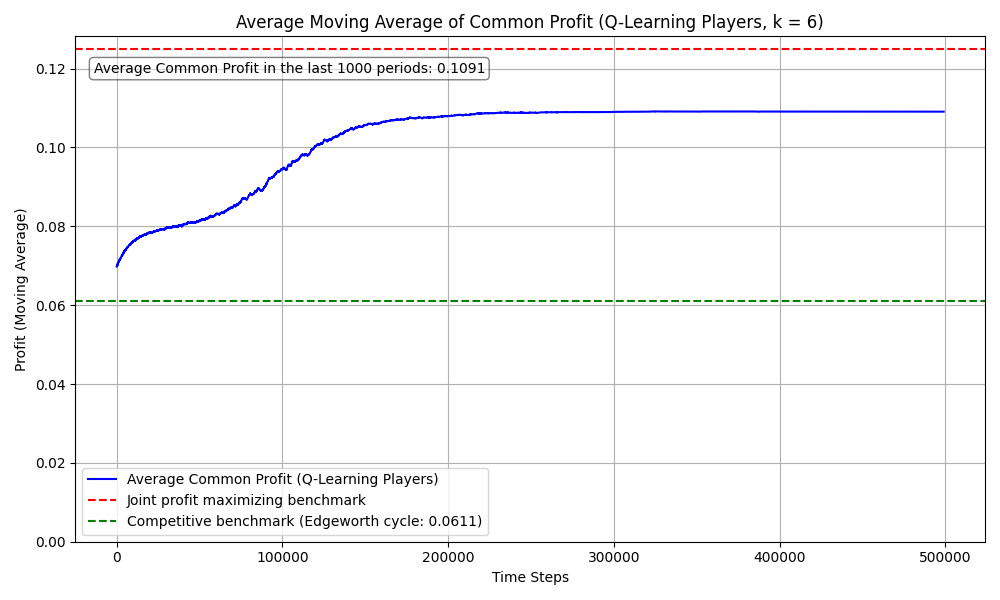
\includegraphics[width=\linewidth]{K=6.png}
        \caption{Q-learner vs Q-learner }
        \label{fig: K = 6}
    \end{minipage}
    \hfill
    \begin{minipage}{0.75\linewidth}
        \centering
        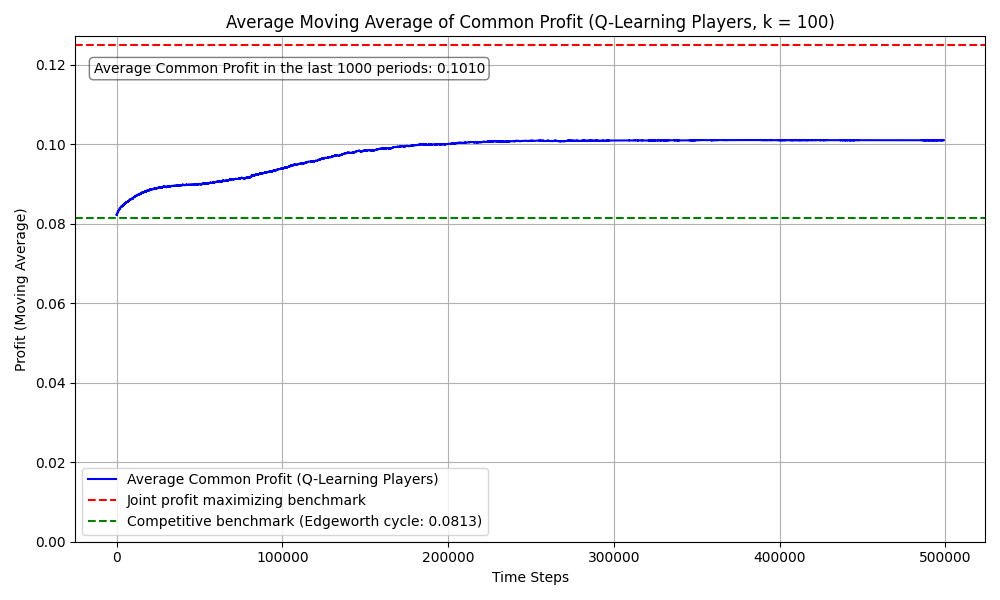
\includegraphics[width=\linewidth]{K=100.png} % Replace with your second image
        \caption{Q-learner vs Q-learner }
        \label{fig: K = 100}
    \end{minipage}
\end{figure}

\subsubsection{Random vs Random}
Figure \ref{fig: RANDOM K = 6} and \ref{fig: RANDOM K = 100} illustrate our simulation results for when two Random players played against each other when K was 6 and 100, respectively. Similar graphs for k values of 12, 24 and 48 can be found in the appendix, in figure \ref{fig:}, \ref{fig:} and \ref{fig: }. This was done by simply having each player sequentially pick a random price with equal probability when it was their turn. Unlike for the Q-learner game, the figures here finely illustrate that no learning is taking place as the plotting of the Average common profit (purple line) does not have any significant fluctuations from start to finish. By our measurements the random players do technically behave collusively, but still not nearly as much as the Q-learner. When comparing the random player figures to the Q-learners, it shows how the Q-learners are learning and converging towards more collusive strategies, while no learning is taking place for the random players.   
\begin{figure}[H]
    \centering
    \begin{minipage}{0.75\linewidth}
        \centering
        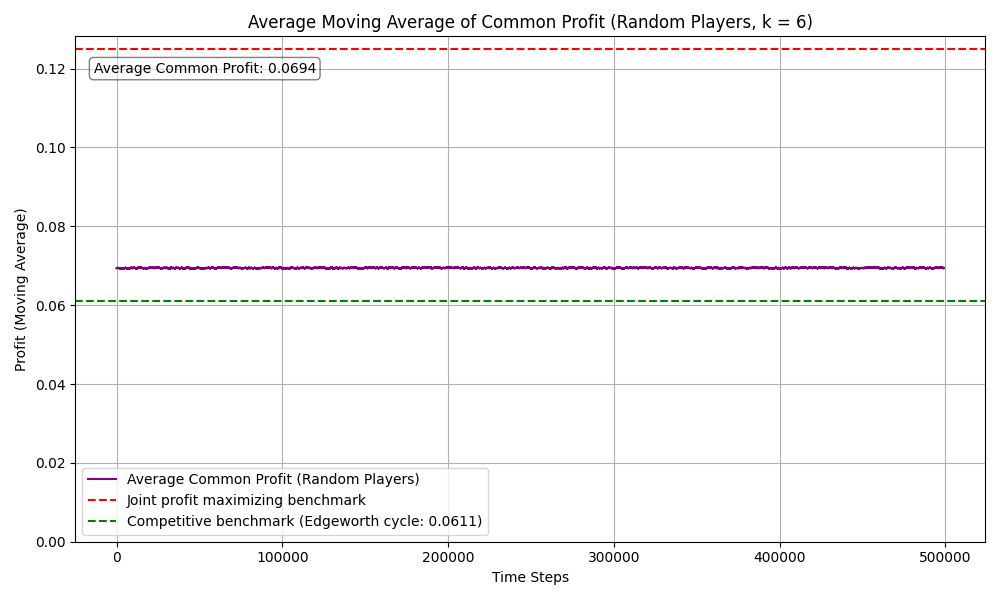
\includegraphics[width=\linewidth]{RANDOM PLAYER, K=6.png}
        \caption{Random players, k = 6 }
        \label{fig: RANDOM K = 6}
    \end{minipage}
    \hfill
    \begin{minipage}{0.75\linewidth}
        \centering
        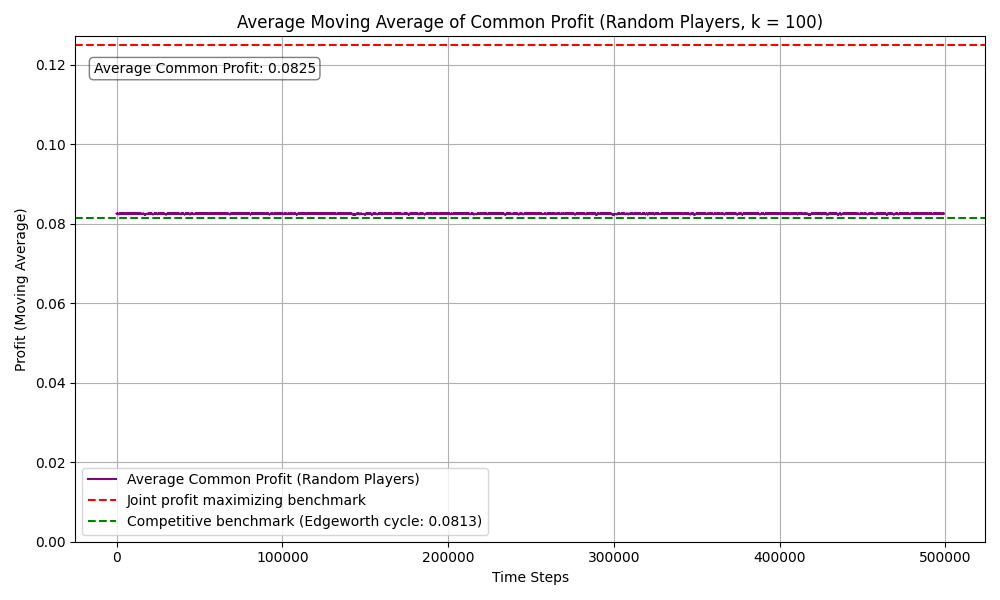
\includegraphics[width=\linewidth]{RANDOM PLAYER, K=100.png}
        \caption{Random players, k = 100}
        \label{fig: RANDOM K = 100}
    \end{minipage}
\end{figure}



\subsubsection{Level of Collusion for K values}
\label{Level of Collusion for K values}

Table \ref{tab:LevelCollusion} shows how much the average profit taken over the last 1000 periods of the runs, lies above the corresponding competitive benchmark, for different values of k. The table is therefore based on the results from section \ref{Q-learning Collusion}. For example, when $k=6$, the Q-learners average profit taken over the last 1000 periods was 78,6$\%$ above the competitive benchmark. 
\begin{table}[H]
    \centering
    \begin{tabular}{|c|c|c|}
        \hline
        \textit{k} & Q-learners & Random players \\
        \hline
        6 & 78.6 \%  & 13.6 \%\\
        \hline
        12 & 46.4 \% & 9.3 \% \\
        \hline 
        24 & 39.2 \% & 5.4 \% \\
        \hline
        48 & 36.6 \% & 2.9 \% \\
        \hline
        100 & 24.2 \% & 1.5 \%\\
        \hline
    \end{tabular}
    \caption{llustrating the percentual deviation between the competetive benchmark and the average profit taken over the last 1000 periods for the Q-learning game and Random game and corresponding k values .}
    \label{tab:LevelCollusion}
\end{table} 
Table \ref{tab:LevelCollusion} highlights the trend which can also be seen in the graphs; as k rises, the profit gets closer to the competitive benchmark. This is the case for both Q-learners and random players. This can arguably be understood as when k increase, the degree of collusive behavior decreases. We can see that for the Q-learner that when k = 6 the average profit of the last 1000 period is 76,8 $\%$ above the competitive benchmark while when k was 100 the Q-learner average common profit over the last 1000 periods was only 24,2$\%$. The trend is also clearly the same for the other k values, 12, 24, and, 48. The table also clearly illustrates (again) the difference in performance between the Q-learning algorithms and the Random Players. 

\subsection{Convergence Analysis}
\label{Convergence Analysis}
In this section we will further investigate what happens when the Q-learning algorithms have converged towards their strategies. Therefore we will look closer at the prices that the different Q-learners are playing in the last periods, to detect if and what cycles arise, or if they end in focal pricing, where both firms repeatedly are setting the same price.

\subsubsection{Overview}

We have written Python code which detects price cycles when the algorithms have converged. We are looking at the last 1000 prices set by the two firms. Notice that we are now investigating the prices set, instead of the profits that the firms are obtaining. 
\newline
The boxplots in figure \ref{fig:Boxplot} is a visualization of the distributions of end-cycle lengths. As \textit{k} grows, the lengths of the cycles grows. This can be seen in both increases in the median and the mean. Furthermore, the longest cycle observed increases with \textit{k}. This is to be expected, as a bigger price interval will allow for more and longer price cycles.
\newline
For all values of \textit{k}, the shortest observed cycle length is 2. These instances constitute focal pricing behavior and, strictly speaking, are not cycles. However, they are identified as such, as both firms repeatedly set the same prices, resulting in what appears to be a cycle of length 2.

\begin{figure}[H]
    \centering
    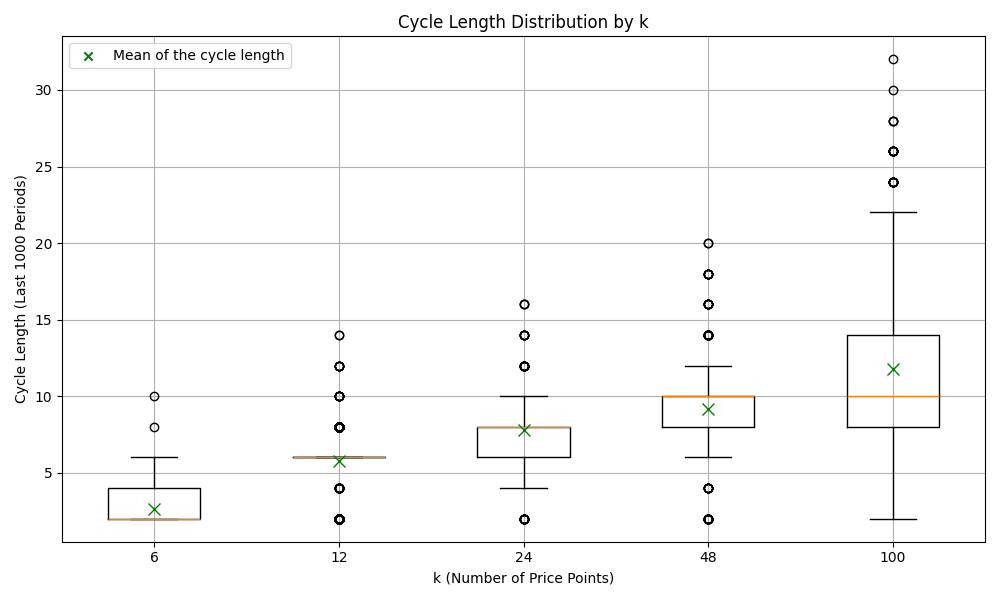
\includegraphics[scale = 0.5]{Boxplotv3.png}
    \caption{Boxplots for the distribution of the cycle lengths in the last 1000 periods for different values of \textit{k}. Notice the mean of the cycle length marked with a green x.}
    \label{fig:Boxplot}
\end{figure}

As the cycles get longer and longer as \textit{k} increases, the share of runs ending with focal pricing decreases. This trend can be seen in figure \ref{fig:ShareFocalPricing}.

\begin{figure}[H]
    \centering
    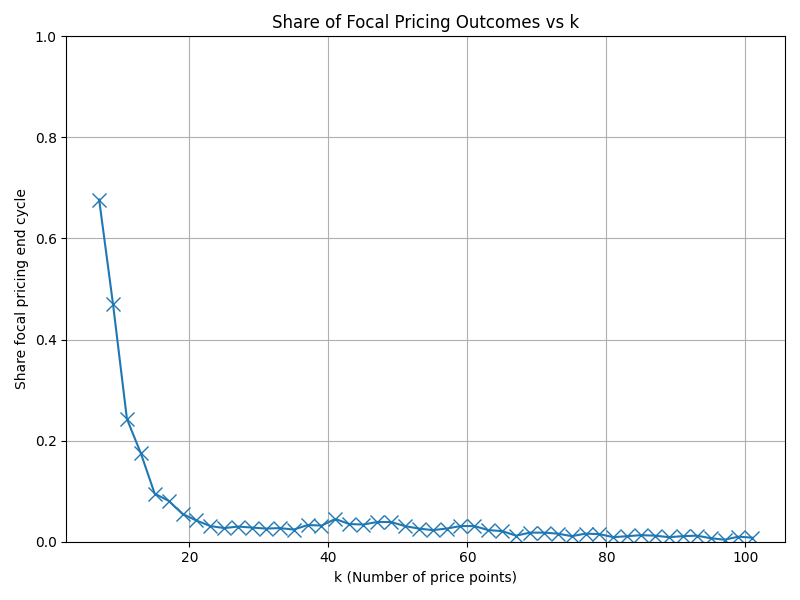
\includegraphics[scale = 0.5]{ShareFocal1000NumRuns.png}
    \caption{Share of focal pricing}
    \label{fig:ShareFocalPricing}
\end{figure}


\subsubsection{In-depth look at cycles}
\label{In-depth look at cycles}


\section{Discussion}


\section{Conclusion}

\newpage 


\section{References}

\bibliographystyle{apalike}
\bibliography{references}


\section{Appendix}
\subsection{Q-learning collusion graphs}

\subsubsection{k = 12}
\begin{figure}[H]
    \centering
    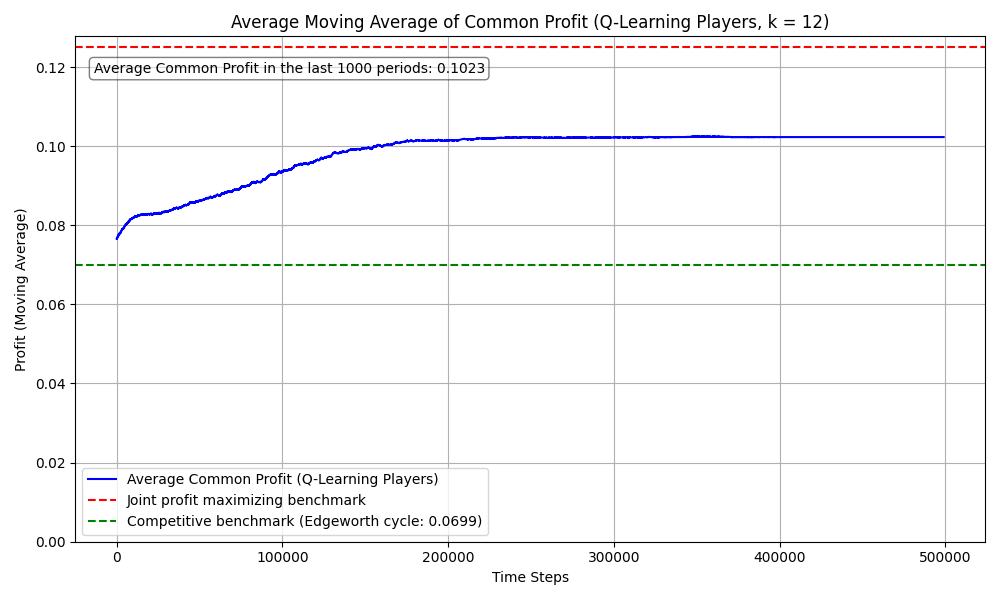
\includegraphics[scale = 0.45]{K=12.png}
    \caption{Q-learner vs Q-learner when k = 12}
    \label{fig: QlearnervQlearnerK=12}
\end{figure}

\subsubsection{k = 24}
\begin{figure}[H]
    \centering
    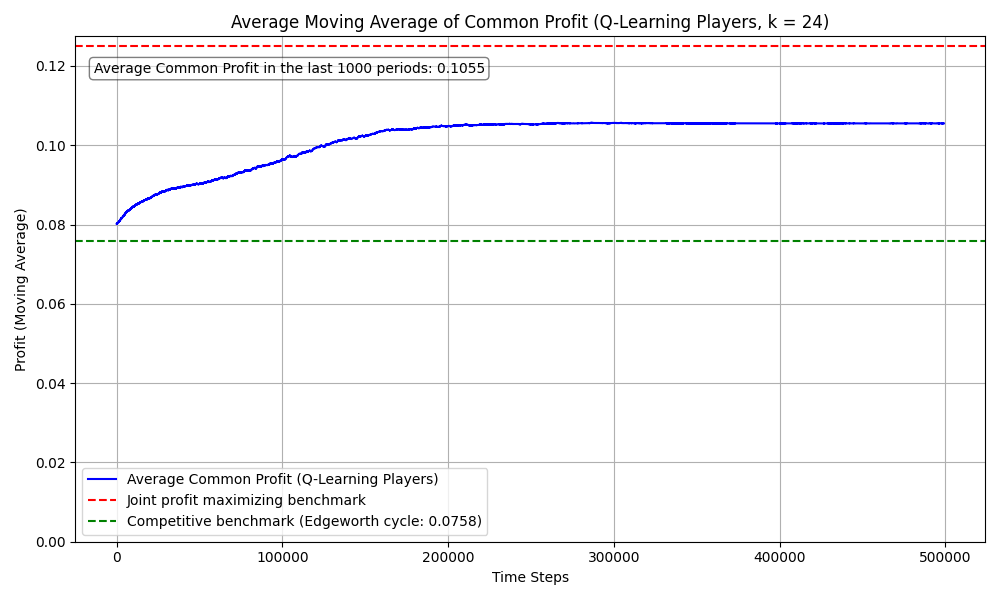
\includegraphics[scale = 0.45]{K=24.png}
    \caption{Q-learner vs Q-learner when k = 24}
    \label{fig: QlearnervQlearnerK=24}
\end{figure}

\subsubsection{k = 48}
\begin{figure}[H]
    \centering
    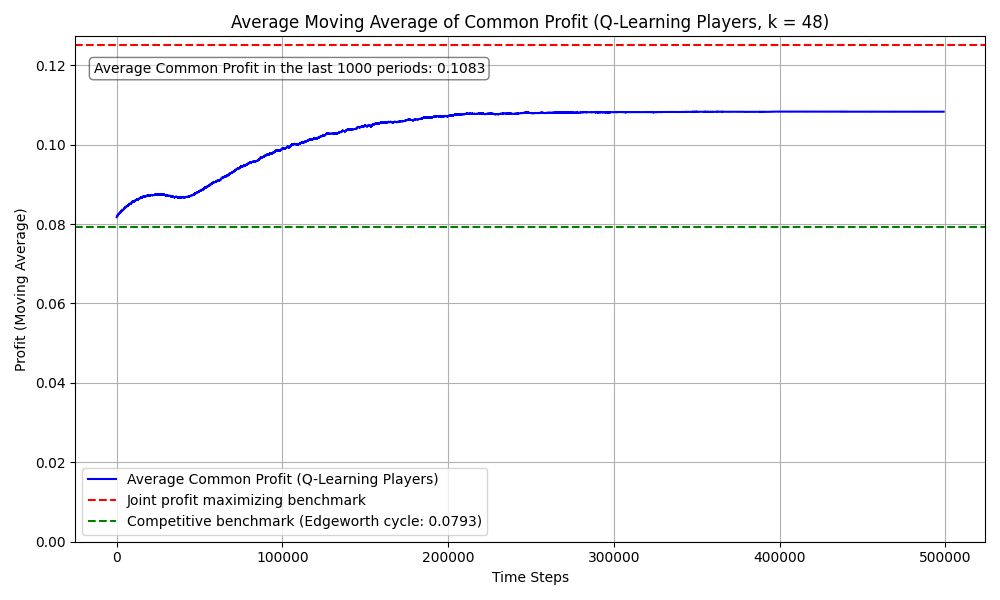
\includegraphics[scale = 0.45]{K=48.png}
    \caption{Q-learner vs Q-learner when k = 48}
    \label{fig: QlearnervQlearnerK=48}
\end{figure}


\end{document}
